\documentclass{article}
\usepackage{graphicx}
\usepackage[margin=1.5cm]{geometry}
\usepackage{amsmath}

\begin{document}
\twocolumn
\title{Warm Up: Conservative Forces}
\author{Prof. Jordan C. Hanson}

\maketitle

\section{Memory Bank}

\begin{itemize}
\item $KE = \frac{1}{2}m v^2$ ... Definition of Kinetic Energy
\item $W = KE_f - KE_i$ ... Work-energy theorem.
\item $U = mgy$ ... Gravitational potential energy, corresponding to $\vec{F} = -mg \hat{j}$.
\item $\vec{F}(x) = -dU/dx ~ \hat{i}$ ... A \textit{conservative force} can be written as the derivative of the potential energy function.  This is the one-dimensional case, where the force only depends on $x$.
\item Let $\oint \vec{F}\cdot d\vec{r}$ represent the integral of $\vec{F}\cdot d\vec{r}$ around a closed path.  A force is \textit{conservative} if
\begin{equation}
\oint \vec{F} \cdot d\vec{r} = 0 \label{eq:1}
\end{equation}
Let $F_x$ represent the x-component of a force $\vec{F}$, and $F_y$ the y-component.  Equation \ref{eq:1} implies that, for a force in the x-y plane,
\begin{equation}
\frac{dF_x}{dy} = \frac{dF_y}{dx}
\end{equation}
\item $KE_i + PE_i = KE_f + PE_f$ ... One form of energy conservation.  Consider that potential energy is just stored energy created by performing work, so this statement is not that different from the official work-energy theorem.
\end{itemize}

\section{Conservative Forces}

\begin{enumerate}
\item In Fig. \ref{fig:1}, we find a potential energy function $U(x) = 2(x^4 - x^2)$. (a) What is the associated force, assumming it is a conservative force? (b) Set the derivative of $U$ equal to zero to locate the points $\pm Q$. (c) What is the potential energy at the points $\pm Q$? (d) If a system with mass $0.1$ kg was released from a distance $dx$ to the right of the origin, what would be the velocity of the system at point Q?  (e) Would that system ever reach $-Q$? \\ \vspace{3cm}
\item Suppose a system of mass 0.1 kg is at the origin, on a surface with coefficient of kinetic friction $\mu = 0.05$.  The system is pushed from $\vec{x} = 0\hat{i}+0\hat{j}$ m, to $\vec{x} = 1\hat{i}+0\hat{j}$ m, then to $\vec{x} = 1\hat{i} + 1\hat{j}$ m, then to $\vec{x} = 0\hat{i} + 1\hat{j}$ m, and finally to $\vec{x} = 0\hat{i}+0\hat{j}$ m.  (a) What is the total work by the pushing force done against friction?  (b) Note that work has been done despite returning to the original position.  Is the friction force conservative?
\end{enumerate}

\begin{figure}
\centering
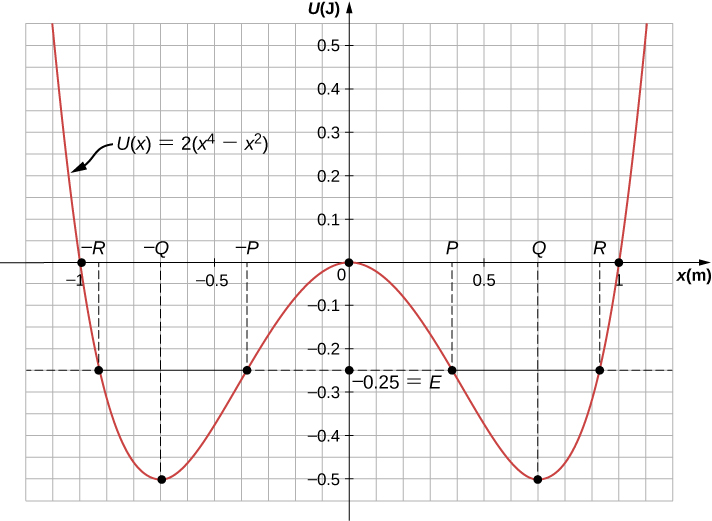
\includegraphics[width=0.33\textwidth]{figures/PE.jpeg}
\caption{\label{fig:1} A function $U(x)$ that describes the potential energy as a function of position.}
\end{figure}

\end{document}
